\documentclass[norsk]{beamer}

\usepackage[framesassubsections]{beamerprosper}
\usepackage[backend=biber, style=alphabetic]{biblatex}
\usepackage{tikz}
\usepackage{tikz-cd}
\usepackage{csquotes}
\usepackage[norsk]{babel}
\usepackage[backend=biber, style=alphabetic]{biblatex}
\usepackage{norsk-thm}

\bibliography{bibliography.bib}

\theoremstyle{example}
\newtheorem{remark}{Bemerkning}

\title{En verden av polynomer}
\author{Jon-Magnus Rosenblad}
\date{13. Mars, 2024}

\begin{document}

\frame{\titlepage}

\frame{\tableofcontents}

\section{Polynomer}

\begin{frame}{Hva er et polynom?}
    Hva er et polynom?
    \begin{definition}
        \[
            a_0 + a_1 x + a_2 x^2 + \dots + a_n x^n
        \]
        hvor $a_0, a_1, \dots, a_n$ er skalarer (varierer ikke med $x$).

        \begin{itemize}
            \item $a_0,\dots, a_n\rightsquigarrow$ \textit{koeffisienter}.
                Kan til eksempel være i $\mathbb Z, \mathbb Q, \mathbb R, \mathbb C$.
            \item $x\rightsquigarrow$ \textit{indeterminant} eller \textit{variabel}.
            \item største $n$ slik at $a_n\neq 0\rightsquigarrow$
                \textit{graden} $n = \deg p$.
        \end{itemize}

        Et polynom kalles \textit{monisk} om $a_n = 1$.

        Mengden av polynomer med Reelle koeffisienter med indeterminant $x$
        benevnes $\mathbb R[x]$.
    \end{definition}
\end{frame}

\begin{frame}{Eksempler}
    \begin{example}
        \begin{itemize}
            \item $p(x) = x^2 + 3x + 2$ er et polynom i $\mathbb R[x]$.
                Det er også et polynom i $\mathbb Z[x]$.
                Det er monisk.
            \item $p(x) = (x + 1)(x + 2)$ er et polynom.
            \item $q(t) = \frac {t^2 + 3t + 2}{t + 1}$ er et polynom av grad $1$,
                $\rightsquigarrow$ det kan skrives som $t + 2$.
                Det ligger i $\mathbb Z[t]$.
        \end{itemize}
    \end{example}
    \begin{example}[Ikke-polynomer]
        \begin{itemize}
            \item $p(x) = \frac{x^2 + 3x + 2}{x - 1}$ er ikke et polynom,
                $\rightsquigarrow$ polynomdivisjon gir
                \[
                    \frac {x^2 + 3x + 2}{x - 1} = x + 4 + \frac 6 {x - 1}
                \]
            \item $p(x) = 3^x$ er ikke et polynom.
        \end{itemize}
    \end{example}
\end{frame}

\begin{frame}{Koeffisienter}
    \begin{figure}
        \centering
        \begin{tikzpicture}
            \begin{scope}[local bounding box=bbox1]
                \draw (0,0) node{$\mathbb Z$}
                    circle (.5)
                    ++(0,.25) node[above=.2cm]{$\mathbb Q$}
                    circle (.8)
                    ++(0,.3) node[above=.5cm]{$\mathbb R$}
                    circle (1.2)
                    ++(0,.3) node[above=.9cm]{$\mathbb C$}
                    circle (1.6);
            \end{scope}
            \begin{scope}[xshift=5cm, local bounding box=bbox2]
                \draw (0,0) node{$\mathbb Z[x]$}
                    circle (.5)
                    ++(0,.25) node[above=.2cm]{$\mathbb Q[x]$}
                    circle (.8)
                    ++(0,.3) node[above=.5cm]{$\mathbb R[x]$}
                    circle (1.2)
                    ++(0,.3) node[above=.9cm]{$\mathbb C[x]$}
                    circle (1.6);
            \end{scope}
            \draw[thick, ->] ([xshift=3pt]bbox1.east) -- ([xshift=(-3pt)]bbox2.west);
        \end{tikzpicture}
    \end{figure}
\end{frame}

\section{Nullpunkter og røtter}

\begin{frame}{Algebraens fundamentalteorem}
    \begin{definition}
        Et tall $x_0$ kalles en \textit{rot} til polynomet $p(x)$
        om $p(x_0) = 0$.
    \end{definition}
    \begin{theorem}[Algebraens fundamentalteorem 1]
        Et polynom $p$ av grad $n$ har ikke flere enn $n$ røtter.
    \end{theorem}
    \pause
    \begin{example}
        \begin{itemize}
            \item $p(x) = x^2 + 4x - 5$ har to røtter: $1, -5$.
            \pause\item $p(x) = x^2 + 4x + 5$ har ingen reelle røtter.
        \end{itemize}
    \end{example}
\end{frame}

\begin{frame}{Faktorisering av polynomer}
    \begin{lemma}
        Om $p(x_0) = 0$, så kan vi faktorisere $p$ som $p(x) = (x - x_0)q(x)$
        for et polynom $q$.
    \end{lemma}
    \pause
    \begin{example}
        La $p(x) = x^3 + 6x^2 + 7x + 6$ har rot $-2$,
        så $(x + 2) | p(x)$.
        \[
            q(x) = \frac {p(x)}{x + 2} = x^2 + 2x + 3
        \]
    \end{example}
\end{frame}

\begin{frame}{Irredusible polynomer}
    \begin{definition}
        Et polynom $p$ kalles \textit{irredusibel} om det går an å faktorisere i
        (ikke-konstante) polynomer.
    \end{definition}
    \begin{remark}
        Her er det viktig at vi skiller mellom om polynomet er over
        $\mathbb Z,\mathbb Q, \mathbb R$ eller $\mathbb C$!
    \end{remark}
    \pause
    \begin{example}
        \begin{itemize}
            \item $x^2 - 2 = (x - \sqrt 2)(x + \sqrt 2)$ er irredusibel over $\mathbb Q$,
                men ikke over $\mathbb R$.
            \item $x^2 + 1 = (x - i)(x + i)$ er irredusibel over $\mathbb R$,
                men ikke over $\mathbb C$. (``Tallet'' $i$ er definert som $\sqrt {-1}$.)
            \item $x^2 - 2\sqrt 2 x + 2 = {(x - \sqrt 2)}^2$ er irredusibelt over $\mathbb Q$,
                men det er ikke heller et polynom over $\mathbb Q$.
        \end{itemize}
    \end{example}
\end{frame}

\begin{frame}{Polynomer over $\mathbb C$}
    \begin{definition}
        De \textit{komplekse tallene} $\mathbb C$ er mengden av
        alle mulige røtter av polynomer med koeffisienter i
        de reelle tallene $\mathbb R$.
    \end{definition}
    \begin{fact}
        Det holder å legge til tallet $i = \sqrt{-1}$ til $\mathbb R$ for å
        få tak i alle røtter!
    \end{fact}
\end{frame}

\begin{frame}{Algebraens fundamentalteorem over $\mathbb C$}
    \begin{theorem}[Algebraens fundamentalteorem]
        Et polynom $p$ av grad $n$ med komplekse koeffisienter kan faktoriseres
        på formen
        \[
            a_n (x - x_1)\dots(x - x_n).
        \]
        En slik faktorisering er unik opp til permutasjon av faktorene.
    \end{theorem}
    \pause
    \begin{corollary}
        Et polynom $p$ av grad $n$ med reelle koeffisienter kan
        faktoriseres på formen
        \[
            p = p_1\dots p_m
        \]
        hvor $p_1,\dots, p_m$ er polynomer av grad høyst $2$.
    \end{corollary}
    \pause
    \begin{remark}
        Vi kan ikke alltid finne alle røttene til et polynom.
        Det beste vi kan håpe på er en faktorisering i irredusible polynomer.
    \end{remark}
\end{frame}

\begin{frame}{Faktorisering av reelle polynomer}
    \begin{example}
        \begin{itemize}
            \item $\begin{aligned}[t]
                    x^3 - 1
                    &= (x - 1)(x^2 + x + 1)
                    \\
                    &= (x - 1)\left(x + \frac{1 + i\sqrt 3} 2\right)\left(x + \frac {1 - i\sqrt 3} 2\right)\end{aligned}$
            \pause\item $\begin{aligned}[t]
                    x^4 + 1
                    &= (x^2 + 2\sqrt 2 + 1)(x^2 - 2\sqrt 2 + 1)\\
                    &=\begin{aligned}[t]
                        &\left(x - \frac {\sqrt 2 + i\sqrt 2}{2}\right)
                        \left(x - \frac {\sqrt 2 - i\sqrt 2}{2}\right)\\
                        &\left(x + \frac {\sqrt 2 + i\sqrt 2}{2}\right)
                        \left(x + \frac {\sqrt 2 - i\sqrt 2}{2}\right)
                    \end{aligned}
                \end{aligned}$
        \end{itemize}
    \end{example}
\end{frame}

\begin{frame}{Kompleks-konjugering}
    \begin{definition}
        La $z = a + ib$ være et komplekst tall, med $i = \sqrt{-1}$.
        Definer den \textit{komplekskonjugerte av $z$} som $\overline z = a - ib$.
    \end{definition}
    \begin{columns}
        \begin{column}{.6\textwidth}
            La $z = a + ib$ og $w = c + id$.
            \begin{itemize}
                \item $\begin{aligned}[t]
                        \overline{(z + w)}
                        &= (a + c) - i(b + d)\\
                        &= \overline z + \overline w
                    \end{aligned}$.
                \pause\item $\begin{aligned}[t]
                        \overline{zw}
                        &= (ac - bd) - i(ad + bc)\\
                        &= \overline{z}\cdot\overline{w}
                    \end{aligned}$.
            \end{itemize}
        \end{column}
        \begin{column}{.4\textwidth}
            \begin{figure}
                \centering
                \begin{tikzpicture}[scale=1.6, point/.style={circle, inner sep=1pt, fill=black}]
                    \draw[lightgray] (-.7, -1.1) grid[step=.2] (1.1, 1.1);
                    \draw[->] (-.8,0) -- (1.2, 0)
                        node[right]{$\mathbb R$};
                    \draw[->] (0, -1.2) -- (0, 1.2)
                        node[above]{$i\mathbb R$};
                    \draw (0.5, {sqrt(3) / 2}) node[point] (z){}
                        node[above right]{$z = a + ib$};
                    \draw (0.5, {-sqrt(3) / 2}) node[point] (zbar){}
                        node[below right]{$\overline z = a - ib$};
                    \draw[dashed] (z) -- (zbar);
                \end{tikzpicture}
            \end{figure}
        \end{column}
    \end{columns}
\end{frame}

\begin{frame}
    \begin{columns}
        \begin{column}{.4\textwidth}
            \begin{itemize}
                \item[$\rightsquigarrow$] $\overline{(x^n)} = \overline x\cdot \overline{(x^{n - 1})} = \overline x^n$ ved induksjon.
                \item[$\rightsquigarrow$] $\overline{p(x)} = p(\overline x)$.
            \end{itemize}
        \end{column}
        \begin{column}{.6\textwidth}
            \begin{figure}
                \centering
                \begin{tikzpicture}[scale=1.6, point/.style={circle, inner sep=1pt, fill=black}]
                    \draw[lightgray] (-1.1, -1.1) grid[step=.2] (1.1, 1.1);
                    \draw[->] (-1.2,0) -- (1.2, 0)
                        node[right]{$\mathbb R$};
                    \draw[->] (0, -1.2) -- (0, 1.2)
                        node[above]{$i\mathbb R$};
                    \draw (45:1) node[point] (r1){}
                        node[above right]{$\frac{\sqrt 2 + i\sqrt 2} 2$};
                    \draw (135:1) node[point] (r2){}
                        node[above left]{$\frac{-\sqrt 2 + i\sqrt 2} 2$};
                    \draw (224:1) node[point] (r3){}
                        node[below left]{$\frac{-\sqrt 2 - i\sqrt 2} 2$};
                    \draw (315:1) node[point] (r4){}
                        node[below right]{$\frac{\sqrt 2 - i\sqrt 2} 2$};
                    \draw (0:.2) arc (0:45:.2)
                        node[midway, above right]{$45^\circ$};
                    \draw (0,0) -- (r1);
                \end{tikzpicture}
                %\caption{Røttene til $x^4 + 1$.}
            \end{figure}
        \end{column}
    \end{columns}
    \begin{proof}[Bevis av korollar]
        Om $p(x_0) = 0$ for et komplekst tall $x_0 = a + ib$,
        så må $p(\overline {x_0}) = \overline 0 = 0$,
        så $(x - x_0)(x - \overline{x_0}) | p(x)$.
        \[\begin{aligned}
            (x - x_0)(x - \overline{x_0})
            &= x^2 - (x_0 + \overline{x_0}) x + x_0\overline{x_0}
            \\
            &= x^2 - 2a x + (a^2 + b^2).
        \end{aligned}\]
    \end{proof}
\end{frame}

\begin{frame}{Hvordan finne polynomrøtter?}
    \begin{lemma}
        Et polynom på formen $ax^2 + bx + c$
        har røtter gitt ved
        \[
            \frac {
                -b \pm \sqrt{b^2 - 4ac}
            }{2a}
        \]
    \end{lemma}
    \pause
    \begin{fact}
        Det finnes en tilsvarende formel for polynomer av grad $3$ og $4$.
    \end{fact}
    \pause
    \begin{columns}
        \begin{column}{.6\textwidth}
            \begin{theorem}[Niels Henrik Abel -- en nordmann]
                Det finnes ingen formel for å finne røttene til et
                generelt polynom av grad $5$ eller høyere.
            \end{theorem}
        \end{column}
        \begin{column}{.25\textwidth}
            \begin{figure}
                \centering
                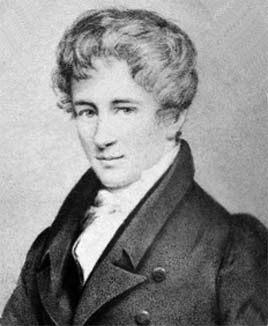
\includegraphics[width=\textwidth]{figures/abel-portrait.jpg}
            \end{figure}
        \end{column}
    \end{columns}
\end{frame}

\begin{frame}{Telle antall røtter}
    Algebraens fundamentalteorem forteller oss at vi kan skrive
    \[
        p = p_1\dots p_m
    \]
    hvor $\deg p_i$ er $1$ eller $2$,
    og $\deg p = \deg p_1 + \dots + \deg p_m$.

    \pause
    \begin{corollary}
        Et polynom av odd grad har minst \'en reell rot.
    \end{corollary}
    \begin{proof}[Bevis 1]
        Minst ett av polynomene $p_1,\dots,p_m$ må være lineært.
    \end{proof}
\end{frame}

\begin{frame}{Skjæringssetningen}
    \begin{lemma}
        La $p(x)$ være et polynom.
        Om det finnes reelle tall $a$ og $b$ slik
        at $a < b$, $p(a) < 0$ og $p(b) > 0$,
        så finnes et tall $c$ slik at
        $a < c < b$ og $p(c) = 0$.
    \end{lemma}
    \begin{figure}
        \centering
        \begin{tikzpicture}[scale = 2, point/.style={inner sep=1pt, circle, fill=black}]
            \draw[lightgray] (-1.1,-1.1) grid[step=.2] (1.1, 1.1);
            \draw[->] (-1.2, 0) -- (1.2,0);
            \draw[->] (0, -1.2) -- (0,1.2);
            \draw[thick, domain=-1:1, samples=20, smooth] plot (\x, {(\x - 1/27)^3 - 1/9});
            \draw (-.5, {(-0.5 - 1/27)^3 - 1/9}) node[point] (pa) {}
                node[right] {$p(a)$};
            \draw (.9, {(0.9 - 1/27)^3 - 1/9}) node[point] (pb) {}
                node[right] {$p(b)$};
            \draw ({1/27 + 1/(3^(2/3))}, 0) node[point] {}
                node[below]{$p(c)$};
            \draw[dashed] (pa) -- (-.5,0)
                node[above]{$a$};
            \draw[dashed] (pb) -- (.9,0)
                node[below]{$b$};
        \end{tikzpicture}
    \end{figure}
\end{frame}

\begin{frame}
    \begin{proof}[Bevis 2]
        Anta $p$ er et monisk odd polynom.
        Da finnes det $a < b$ slik at $p(a) < 0$ og $p(b) > 0$,
        så ved skjæringssetningen må det finnes en rot mellom $a$ og $b$.
    \end{proof}
    \begin{figure}
        \centering
        \begin{tikzpicture}
            \draw[lightgray] (-2.1, -2.1) grid[step=.5] (2.1, 2.1);
            \draw[->] (-2.2,0) -- (2.2, 0);
            \draw[->] (0, -2.2) -- (0, 2.2);
            \draw[thick, domain=-2:2, samples=20, smooth] plot (\x, {(\x^3 - \x) / 3})
                node[right] {$\frac 1 3(x^3 - x)$};
        \end{tikzpicture}
    \end{figure}
\end{frame}

\section{Rasjonale røtter}

\begin{frame}{Skjæringssetningen for rasjonale polynomer}
    \begin{remark}
        Skjæringssetningen holder ikke over de rasjonale tallene!
    \end{remark}
    \begin{example}
        Polynomet $p(x) = x^3 - \frac 1 2$ skjærer ikke $x$-aksen i et rasjonalt punkt.
        \begin{figure}
            \centering
            \begin{tikzpicture}[scale=2]
                \draw[thin, lightgray] (-.7,-.9) grid[step=.2] (1.1, .5);
                \draw[->] (-.8, 0) -- (1.2, 0);
                \draw[->] (0,-1) -- (0,.6);
                \draw[thick, domain=-.6:1, samples=20, smooth] plot (\x, {\x^3 - 1/2});
                \draw ({2^(-1/3)}, 0)
                    node[circle, inner sep=1pt, fill=black] {}
                    node[below right] {$\left(\frac {1}{\sqrt[3] 2}, 0\right)$};
            \end{tikzpicture}
        \end{figure}
    \end{example}
\end{frame}

\begin{frame}{Heltallige og rasjonale polynomer}
    \begin{lemma}
        La $p(x)$ være et rasjonalt polynom.
        Om $p$ er redusibel over $\mathbb Q$,
        så finnes det et heltall $m \gg 0$ slik at
        $mp(x)$ er redusibel over $\mathbb Z$.
    \end{lemma}
    \begin{example}
        \begin{itemize}
            \item $x^2 - \frac 1 4$
                kan faktoriseres som $\frac 1 4 \underbrace{(2x - 1)(2x + 1)}_{4x^2 - 1}$.
        \end{itemize}
    \end{example}
    \pause
    \begin{theorem}
        La $p(x)$ være et monisk polynom med heltallige koeffisienter.
        Om det finnes et rasjonalt tall $x_0$ slik at
        $p(x_0) = 0$, så må $x_0$ være et heltall.
    \end{theorem}
\end{frame}

\begin{frame}{Eisensteins kriterium}
    \begin{theorem}[{Eisensteins kriterium \cite[Oppgave~3.12]{polynomials}}]
        La $h(x) = a_n x^n + \dots + a_1 x + a_0$ være et polynom over $\mathbb Z$.
        Om det finnes et primtall $p$
        slikt at
        \begin{itemize}
            \item $p\nmid a_n$,
            \item $p | a_0,\dots, a_{n -  1}$,
            \item $p^2 \nmid a_0$,
        \end{itemize}
        da er $h$ irredusibel over $\mathbb Z$.
    \end{theorem}
    \begin{example}
        Polynomet $x^n - p$ er irredusibel over $\mathbb Z$ (og $\mathbb Q$ for alle heltall $n$ og primtall $p$.
        Over $\mathbb R$ kan det faktoriseres som
        \[
            x^n - p = (x - \sqrt[n] p) (x^{n - 1} + \sqrt[n] p x^{n - 1} + \dots + \sqrt [n] p^{n - 1}).
        \]
    \end{example}
\end{frame}

\begin{frame}{Mengden av røtter}
    Hvilke tall trenger vi å ha med for å dele opp alle rasjonale
    polynomer i lineære polynomer? $\rightsquigarrow \overline{\mathbb Q}$
    \begin{columns}
        \begin{column}{.6\textwidth}
            \begin{itemize}
                \item $x^2 - 2$ $\rightsquigarrow$ $\sqrt 2$ er i $\overline{\mathbb Q}$,
                    men ikke i $\mathbb Q(i)$.
                \item $x^2 + 1$ $\rightsquigarrow$ $i = \sqrt{-1}$ er i $\overline{\mathbb Q}$,
                    men ikke i $\mathbb R$.
                \item Det er ingen rasjonale polynomer med $\pi$ som rot,
                    så $\pi$ er ikke i $\overline{\mathbb Q}$.
            \end{itemize}
            \begin{remark}
                Det finnes ingen endelig mengde elementer vi kan legge til for å få alle
                røtter av rasjonale polynomer.
            \end{remark}
        \end{column}
        \begin{column}{.4\textwidth}
            \begin{figure}
                \centering
                \begin{tikzpicture}
                    \draw (0,0) node{$\mathbb Q$}
                        +(0,-.3)
                        circle (.8)
                        node[below=.3cm]{$\mathbb R$}
                        ++(0,.3) node[above=.2cm]{$\mathbb Q(i)$}
                        circle (.8)
                        ++(0,.3) node[above=.5cm]{$\overline{\mathbb Q}$}
                        circle (1.2)
                        node[above=1.2cm]{$\mathbb C$}
                        circle (1.8);
                \end{tikzpicture}
            \end{figure}
        \end{column}
    \end{columns}
\end{frame}

\section{Polynomer i flere variable}

\begin{frame}{Polynomer i $2$ variable}
    \begin{definition}
        Et polynom i to variable $p(x,y)$
        er et polynom i \'en variabel $x$ hvor koeffisientene
        er polynomer i en annen variabel $y$
        \[
            p(x, y) = p_n(y) x^n + \dots + p_1(y) x + p_1(y).
        \]

        Graden til polynomet er den største summen av grader
        $i + \deg p_i$.
    \end{definition}
    \begin{example}
        \begin{itemize}
            \item $x^2 + y^2 - 9$
            \item $x_1^2 + x_2^2 - 9$ er det samme polynomet,
                men indeterminantene er gitt ved andre symboler.
        \end{itemize}
    \end{example}
\end{frame}

\begin{frame}{Implisitte kurver og parametrisering}
    \begin{definition}
        En \textit{implisitt kurve $C$ i planet $\mathbb R^2$}
        er en mengde på formen
        \[
            C = \{ (x,y)\in \mathbb R^2 \mid p(x,y) = 0\},
        \]
        hvor $p$ er et polynom,
        dvs. $C$ er mengden av løsninger til likningen $p(x,y) = 0$.
    \end{definition}
    \begin{columns}
        \begin{column}{.4\textwidth}
            \begin{remark}
                En implisitt kurve er ``nullpunktsmengden'' til et polynom.
            \end{remark}
        \end{column}
        \begin{column}{.6\textwidth}
            \begin{figure}
                \centering
                \begin{tikzpicture}[scale=1.6]
                    \draw[lightgray] (-1.1,-1.1) grid[step=.2] (1.1, 1.1);
                    \draw[->] (-1.2,0) -- (1.2,0);
                    \draw[->] (0,-1.2) -- (0,1.2);
                    \draw[thick, domain=0:360, samples=36, smooth] plot ({cos(\x)},{sin(\x)});
                    \draw (45:1) node[above right] {$\{x^2 + y^2 - 1 = 0\}$};
                \end{tikzpicture}
            \end{figure}
        \end{column}
    \end{columns}
\end{frame}

\begin{frame}{Irredusible polynomer i $2$ variable}
    \begin{definition}
        Et polynom $p(x,y)$ er irredusibel om det ikke kan skrives
        som et produkt av polynomer av lavere grad.
    \end{definition}
    \begin{columns}
        \begin{column}{.5\textwidth}
            \begin{itemize}
                \item $x^2 + y^2 - 1$ er irredusibel.
                \item $x^2 - y^2 = (x - y)(x + y)$.
                \pause\item $x^4 - x^2 y^2 - x^2 y + y^3 - \frac 3 4 x^2 + y^2 + \frac 1 4 y + \frac 1 4$?
            \end{itemize}
        \end{column}
        \begin{column}{.5\textwidth}
            \pause
            \begin{figure}
                \centering
                \begin{tikzpicture}[scale=.8]
                    \draw[lightgray] (-3.1, -3.1) grid[step=.5] (3.1, 3.1);
                    \draw[->] (-3.2,0) -- (3.2,0);
                    \draw[->] (0,-3.2) -- (0,3.2);
                    \draw[thick, samples=20, smooth, domain=-2:2]
                        plot (\x, {(\x)^2 - 1});
                    \draw[thick, samples=20, smooth, domain=-3:3]
                        plot ({sqrt((\x)^2 + 1/4)}, \x)
                        plot ({-sqrt((\x)^2 + 1/4)}, \x);
                \end{tikzpicture}
            \end{figure}
        \end{column}
    \end{columns}
\end{frame}

\begin{frame}
    \begin{figure}
        \centering
        \begin{tikzpicture}[scale=.8]
            \draw[lightgray] (-3.1, -3.1) grid[step=.5] (3.1, 3.1);
            \draw[->] (-3.2,0) -- (3.2,0);
            \draw[->] (0,-3.2) -- (0,3.2);
            \draw[red, thick, samples=20, smooth, domain=-2:2]
                plot (\x, {(\x)^2 - 1})
                node[above] {$y = x^2 - 1$};
            \draw[blue, thick, samples=20, smooth, domain=-3:3]
                plot ({sqrt((\x)^2 + 1/4)}, \x)
                node[below right] {$x^2 - y^2 - \frac 1 4 = 0$}
                plot ({-sqrt((\x)^2 + 1/4)}, \x);
        \end{tikzpicture}
    \end{figure}
    \pause
    \begin{multline*}
        x^4 - x^2 y^2 - x^2 y + y^3 - \frac 3 4 x^2 + y^2 + \frac 1 4 y + \frac 1 4
        \\
        = \left(x^2 - y^2 - \frac 1 4\right)(x^2 - 1 - y).
    \end{multline*}
\end{frame}

\frame{\printbibliography}

\end{document}
